\chapter{Experiments}
\section{Experiments}
In this section, we present the results obtained from applying the autotuning and recommendation policies described in Section 6, to our target applications --- AmberMD, SNAP, 3DStencil, and MiniAMR. We describe results from a study of overheads involved in enabling MPI\_T in MVAPICH2 and TAU.

\subsection{Experimental Setup}
Our experiments with AmberMD, SNAP, and 3DStencil were performed on Stampede, a 6400 node Infiniband cluster at the Texas Advanced Computing Center~\cite{TACC}. Each regular Stampede compute node has two Xeon E5-2680 8-core \quotes{Sandy Bridge} processors and one first-generation Intel Xeon Phi SE10P KNC MIC. We chose to run all our experiments using pure MPI on the Xeon host with 16 MPI processes on a node (1 per core) with \verb+MV2_ENABLE_AFFINITY+ turned on so that MPI tasks were pinned to CPU cores. For SNAP, we used a total of 64 nodes (at 16 processes per node, a total of 1024 processes). For our experiments with AmberMD and 3DStencil, we used a total of 32 nodes (at 16 processes per node, a total of 512 processes). \par
Experiments with MiniAMR and those involving a study of sampling overheads using 3DStencil were performed on the ri2 Infiniband cluster at The Ohio State University. Each compute node on ri2 has two 14-core Intel Xeon E5-2680 v4 processors. The HCA on all nodes in the cluster is the Mellanox CX-4 100 Gigabit adapter. The OFED version used is MLNX\_OFED\_LINUX-4.1-1.0.2.0 and the Linux kernel version is 3.10.0-327.10.1.el7.x86\_64. We ran all our experiments using pure MPI on Intel Xeon hosts with 28 MPI processes on a node (1 per core) and pinned the MPI processes. We used a total of 2-16 nodes (at 28 processes per node, a total of 56 to 448 processes) for our experiments with 3DStencil, and a total of 8 nodes (at 28 processes per node, a total of 224 processes) for experiments with MiniAMR.

\subsection{Results}

\subsubsection{Amber}
Table \ref{tab:Amber} summarizes the results of modifying the \emph{Eager} threshold and applying the runtime autotuning policy for AmberMD.
The threshold is set statically right after MPI initialization, using \verb+MPIR_CVAR_IBA_EAGER_THRESHOLD+.
We noted that increasing the \emph{Eager} threshold from the MVAPICH2 default value to 64000 bytes had the effect of reducing application runtime by 19.2\%. This was achieved at the cost of increasing the total VBUF memory across all processes by 320\%. Please note that the total VBUF memory usage reported here is the \textit{average} value across the number of times that this metric was sampled (once every 10 seconds). The third row shows results of applying the user-defined policy of freeing unused VBUFs at runtime, on top of the \emph{Eager} threshold optimization. We saw a sizeable reduction in total VBUF memory used while the runtime remained unaffected.

\subsubsection{SNAP}
SNAP application relies heavily on point-to-point communication, and the message sizes involved in communication depend on a number of input factors. We followed the recommended ranges for these input factors:
\begin{itemize}
\item Number of angles per octant (nang) was set to 50
\item Number of energy groups (ng) was set to 150
\item Number of spatial cells per MPI rank was set to 1200
\item Scattering order (nmom) was set to 4
\end{itemize}
We gathered the message sizes involved in MPI communication. Table \ref{tab:SNAP_profile} lists the five MPI functions that account for the highest aggregate time spent. \verb+MPI_Recv+ and \verb+MPI_Waitall+ together account for nearly 17\% of total application time or 60\% of MPI time. Table \ref{tab:SNAP_message_sizes} lists the message sizes involved in various MPI routines. It is evident that the bulk of messages are point-to-point messages with a message size of roughly 18,300 bytes. \par
The fact that the application spends a lot of its communication time inside \verb+MPI_Recv+ (callsite ID 5 in Table \ref{tab:SNAP_profile}) and \verb+MPI_Waitall+ (callsite ID 16 in Table \ref{tab:SNAP_profile}) suggests that the receiver in the point-to-point communication is generally late as compared to the posting of the corresponding \verb+MPI_Isend+ (callsite ID 1 in Table \ref{tab:SNAP_profile}) operation. As a result of the relatively large message size of 18KB involved in this case, the data is transferred using the Rendezvous protocol \textit{after} the receive is posted --- in this specific context, this data transfer happens when the sender reaches the \verb+MPI_Waitall+ call. Even though there is an opportunity for communication-computation overlap through the use of non-blocking routines, no overlap actually happens in the application because of the conditions necessary for the transfer of large messages using the Rendezvous protocol. \par
By increasing both the inter-node and intra-node Eager threshold to 20KB, the transfer of these point-to-point messages is initiated when the sender posts the \verb+MPI_Isend+ operation. As a result, the application sees an increase in communication-computation overlap, and this manifests itself as a reduction in overall application runtime. The second row of Table \ref{tab:SNAP} summarizes this improvement in performance with 1024 processes --- we note a reduction of 10.7\% in application runtime when increasing the Eager threshold to 20 KB. However, increasing the Eager threshold also meant that the total VBUF memory usage across all processes went up by 12\%. \par
The TAU autotuning plugin ensures that VBUFs from unused pools are freed to offset this increase in total VBUF memory usage. The third row of Table \ref{tab:SNAP} summarizes the reduction in total VBUF memory usage when the TAU autotuning plugin is enabled. It is important to note that the plugin does not disturb application runtime even at this scale.

\subsubsection{3DStencil}
Table \ref{tab:3DStencil} summarizes the results of these experiments with our synthetic 3DStencil code. We designed the application in such a way that non-blocking point-to-point communications involve messages of an arbitrarily high, but fixed size. We measured the communication-computation overlap achieved. The first row describes results for the default run, where a very low communication-computation ratio of 6.0\% was achieved as messages are sent using the \emph{Rendezvous} protocol. The reason for setting a high, but fixed value for message size was to ensure that only VBUFs from one pool are utilized. In a manner similar to AmberMD, this application benefited from an increased value for the \emph{Eager} threshold. The communication-computation ratio went up from 4.6\% to 79.9\% and as a result, there was a corresponding drop in application runtime by 26.2\%. However, the total VBUF memory utilized went up by 1.6 times as compared to the default setup. We noted significant benefits in implementing the runtime autotuning policy of freeing unused VBUFs, although it still was 1.49 times of the original. \par

It is important to note that the actual amount of memory freed through the autotuning logic depends on the usage levels of various pools. With both AmberMD and 3DStencil, the message sizes involved in the communication were relatively large --- as a result, smaller size VBUFs were freed.

\subsubsection{MiniAMR}
Table \ref{tab:MiniAMR} summarizes the results of enabling SHArP for MiniAMR. Both the default and optimized runs were performed under similar conditions, with increased values for check-summing frequency and stages per timesteps to better demonstrate the potential benefits of enabling hardware offloading of collectives. Under these conditions, we saw an improvement of 4.6\% in runtime when enabling SHArP on 8 nodes. 

\begin{table*}[!tbp]
  \centering
  \small
  \captionsetup{justification=centering}
  \caption{AmberMD - Impact of Eager threshold and autotuning on execution time and memory usage}
  \label{tab:Amber}
  \resizebox{\columnwidth}{!}{\begin{tabular}{|c|c|c|c|c|l|}
    \toprule
    Run& \begin{tabular}{@{}c@{}}Number of \\ Processes\end{tabular} & \begin{tabular}{@{}c@{}} Eager \\ Threshold \\ (Bytes)\end{tabular} & Timesteps& \begin{tabular}{@{}c@{}}Runtime \\ (secs)\end{tabular} & \begin{tabular}{@{}c@{}}Total \\ VBUF \\ Memory(KB)\end{tabular}\\
    \midrule
    Default&512&MVAPICH2 Default&8,000&166&4,796,067\\
    Eager&512&64,000&8,000&134&15,408,619\\
    TAU autotuning&512&64,000&8,000&134&15,240,073\\
  \bottomrule
\end{tabular}}
\end{table*}

\begin{table*}[!tbp]
  \centering
  \small
  \captionsetup{justification=centering}
  \caption{SNAP - Aggregate time inside various MPI functions (top five by total time)}
  \label{tab:SNAP_profile}
  \resizebox{\columnwidth}{!}{\begin{tabular}{|c|c|c|l|}
    \toprule
    MPI routine name&\begin{tabular}{@{}c@{}}Callsite ID \end{tabular} &  \begin{tabular}{@{}c@{}}Portion of \\ Application Runtime (\%)\end{tabular} & \begin{tabular}{@{}c@{}} Portion of MPI Time (\%)\end{tabular}\\
    \midrule
    MPI\_Recv&4&13.31&47.50\\
    MPI\_Barrier&5&5.20&18.55\\
    MPI\_Allreduce&7&3.84&13.72\\
    MPI\_Waitall&16&3.09&11.02\\
    MPI\_Isend&1&1.21&4.33\\
  \bottomrule
\end{tabular}}
\end{table*}

\begin{table*}[!tbp]
  \centering
  \small
  \captionsetup{justification=centering}
  \caption{SNAP - Average sent message sizes from various MPI functions (top five by message count)}
  \label{tab:SNAP_message_sizes}
  \resizebox{0.80\columnwidth}{!}{\begin{tabular}{|c|c|c|l|}
    \toprule
    MPI routine name&\begin{tabular}{@{}c@{}}Callsite ID \end{tabular} & \begin{tabular}{@{}c@{}}Count\end{tabular} & \begin{tabular}{@{}c@{}} Average Message Size (Bytes)\end{tabular}\\
    \midrule
    MPI\_Isend&1&114348672&18300\\
    MPI\_Allreduce&7&25600&1200\\
    MPI\_Send&18&2400&1920\\
    MPI\_Bcast&11&1024&120\\
    MPI\_Bcast&15&1024&120\\
  \bottomrule
\end{tabular}}
\end{table*}

\begin{table*}[!tbp]
  \centering
  \small
  \captionsetup{justification=centering}
  \caption{SNAP - Impact of Eager threshold and autotuning on execution time and memory usage}
  \label{tab:SNAP}
  \resizebox{\columnwidth}{!}{\begin{tabular}{|c|c|c|c|l|}
    \toprule
    Run& \begin{tabular}{@{}c@{}}Number of \\ Processes\end{tabular} & \begin{tabular}{@{}c@{}} Eager \\ Threshold (Bytes)\end{tabular} & \begin{tabular}{@{}c@{}}Runtime (secs)\end{tabular} & \begin{tabular}{@{}c@{}}Total VBUF Memory(KB)\end{tabular}\\
    \midrule
    Default&1024&MVAPICH2 Default&47.3&3,322,067\\
    Eager&1024&20,000&42.2&3,787,050\\
    TAU autotuning&1024&20,000&42.9&2,063,421\\
  \bottomrule
\end{tabular}}
\end{table*}

\begin{table*}[!htbp]
  \centering
  \small
  \captionsetup{justification=centering}
  \caption{3DStencil - Impact of Eager threshold and autotuning on execution time and memory usage}
  \label{tab:3DStencil}
  \resizebox{\columnwidth}{!}{\begin{tabular}{|c|c|c|c|c|c|l|}
    \toprule
    Run& \begin{tabular}{@{}c@{}}Number of \\ Processes\end{tabular} & \begin{tabular}{@{}c@{}}Message \\ Size \\ (Bytes)\end{tabular} & \begin{tabular}{@{}c@{}}Eager \\ Threshold \\ (Bytes)\end{tabular} & \begin{tabular}{@{}c@{}}Overlap \\ (\%) \end{tabular}& \begin{tabular}{@{}c@{}}Runtime \\ (secs)\end{tabular} & \begin{tabular}{@{}c@{}}Total \\ VBUF \\ Memory(KB)\end{tabular}\\
    \midrule
    Default&512&32,768&MVAPICH2 Default&4.6&198.1&3,112,302\\
    Eager&512&32,768&33,000&79.9&146.6&4,893,712\\
    TAU autotuning &512&32,768&33,000&80.0&146.4&4,644,691\\
  \bottomrule
\end{tabular}}
\end{table*}

\begin{table*}[!htbp]
  \centering
  \small
  \captionsetup{justification=centering}
  \caption{MiniAMR - Impact of hardware offloading on application runtime}
  \label{tab:MiniAMR}
  \resizebox{0.65\columnwidth}{!}{\begin{tabular}{|c|c|l|}
    \toprule
    Run&Number of Processes&Runtime (secs)\\
    \midrule
    Default&224&648\\
    SHArP enabled&224&618\\
  \bottomrule
\end{tabular}}
\end{table*}


\subsection{Overhead in Enabling MPI\_T}
MVAPICH2 does not enable tracking of MPI\_T PVARs by default. This feature is enabled by configuring MVAPICH2 with the \verb+--enable-mpit-pvars+ flag. Enabling and tracking PVARs has a cost associated with it, and we sought to quantify this cost for small-scale experiments using our infrastructure. Recall that when TAU is configured to track PVARs, TAU samples PVARs at regular intervals --- the default value for the sampling interval is 10 seconds. TAU reads every PVAR exposed by the MPI implementation --- this implies that the overhead with sampling is directly proportional to the number of the PVARs exported. 
\par Using a version of MVAPICH2 with MPI\_T disabled as the baseline, we set up experiments to measure the following overheads:
\begin{itemize}
	\item Overhead of enabling MPI\_T within MVAPICH2
	\item Overhead of sampling PVARs at regular intervals using TAU
\end{itemize}
In our first set of experiments, we sought to quantify the cost of enabling MPI\_T within MVAPICH2, and the cost of sampling at the default rate inside TAU (once every 10 seconds). We measured the execution time for the 3DStencil application on the ri2 cluster --- with 28 MPI processes per node, we ran experiments using 2 to 16 nodes. Each experiment was repeated 5 times, and the average execution time was calculated. The results of these experiments are depicted in Figure \ref{fig:overheads}. 
\par At small-scale, we see negligible overheads with our infrastructure. The execution times for MVAPICH2 configured with MPI\_T are nearly identical to the execution times for the baseline. When sampling at the default rate of once every 10 seconds, TAU's sampling system does not seem to add any noticeable overhead to the execution time --- we see a maximum of 4.7\% overheads when using 2 nodes. With other node counts, the overheads are low enough to be indistinguishable from the run-to-run variability that is dependent on non-deterministic factors.\par In our second set of experiments, we studied how runtime is affected by sampling more frequently from the MPI\_T interface. We measured the execution time of the 3DStencil application on the ri2 cluster using 16 nodes (at 28 processes per node, a total of 448 processes). Each experiment was repeated 5 times, and the average execution time was calculated --- we have not presented the error bars with the results because there was negligible variation between runs. Figure \ref{fig:sampling_frequency} shows that the overheads are negligible even when sampling at a rate of once every second. In summary, the overall runtime for the 3DStencil application is not affected noticeably when the sampling rate is increased. Although it may not be the most suitable method for all usage scenarios, this study suggests that sampling provides a low-overhead solution for tracking PVARs. These experiments suggest that our infrastructure is likely to scale to large node counts. Overhead studies with large node counts will be part of our future work.
\begin{center}
        \begin{figure*}[tbp!]
                 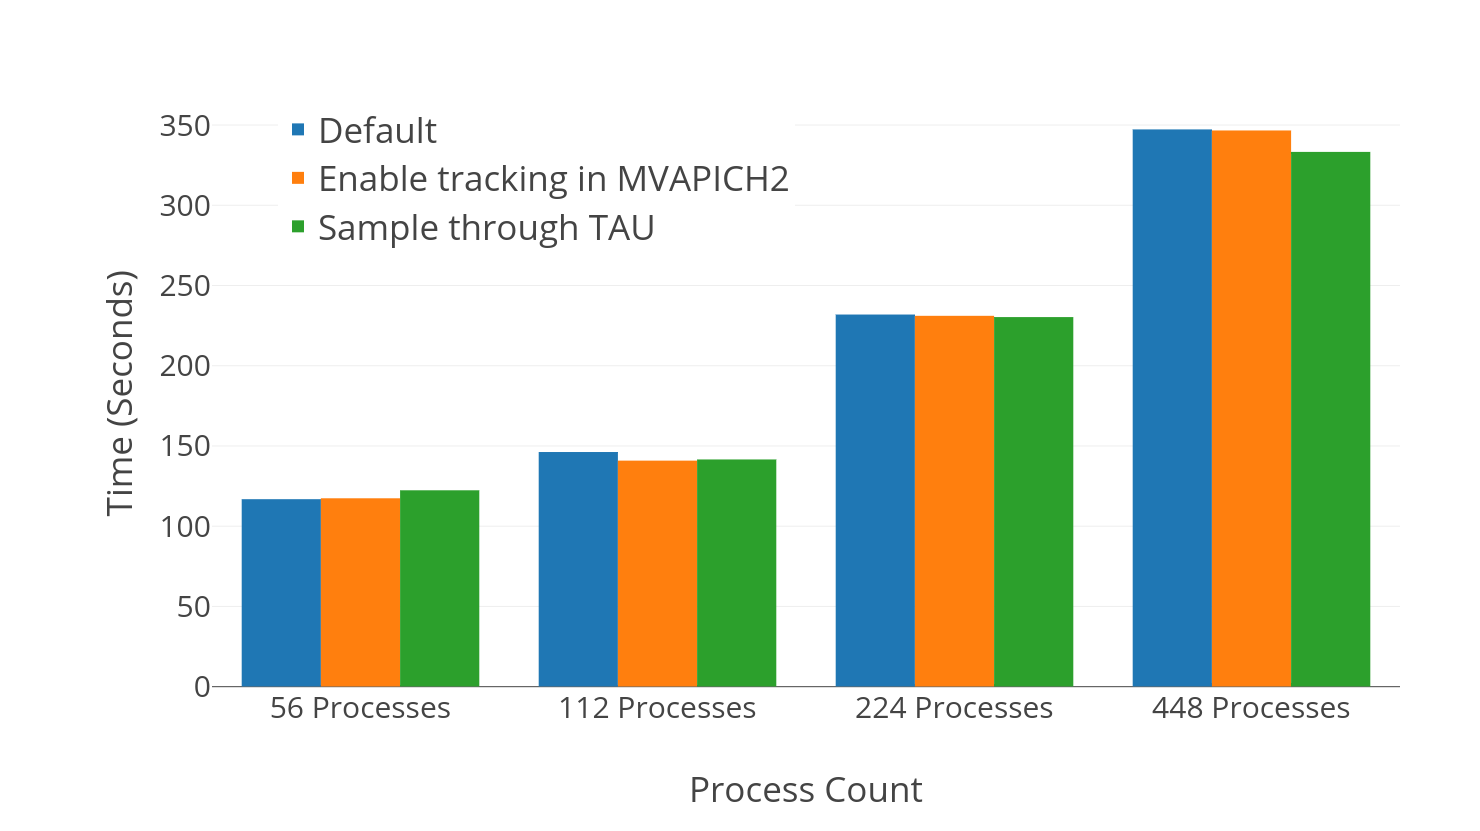
\includegraphics[width=\columnwidth,keepaspectratio,scale=1.0]{figures/MPI_T_Overheads}
                \captionsetup{justification=centering}
                  \caption{Overhead in Enabling MPI\_T for 3DStencil}
                   \label{fig:overheads}
        \end{figure*}
\end{center}


\begin{center}
        \begin{figure*}[tbp!]
                 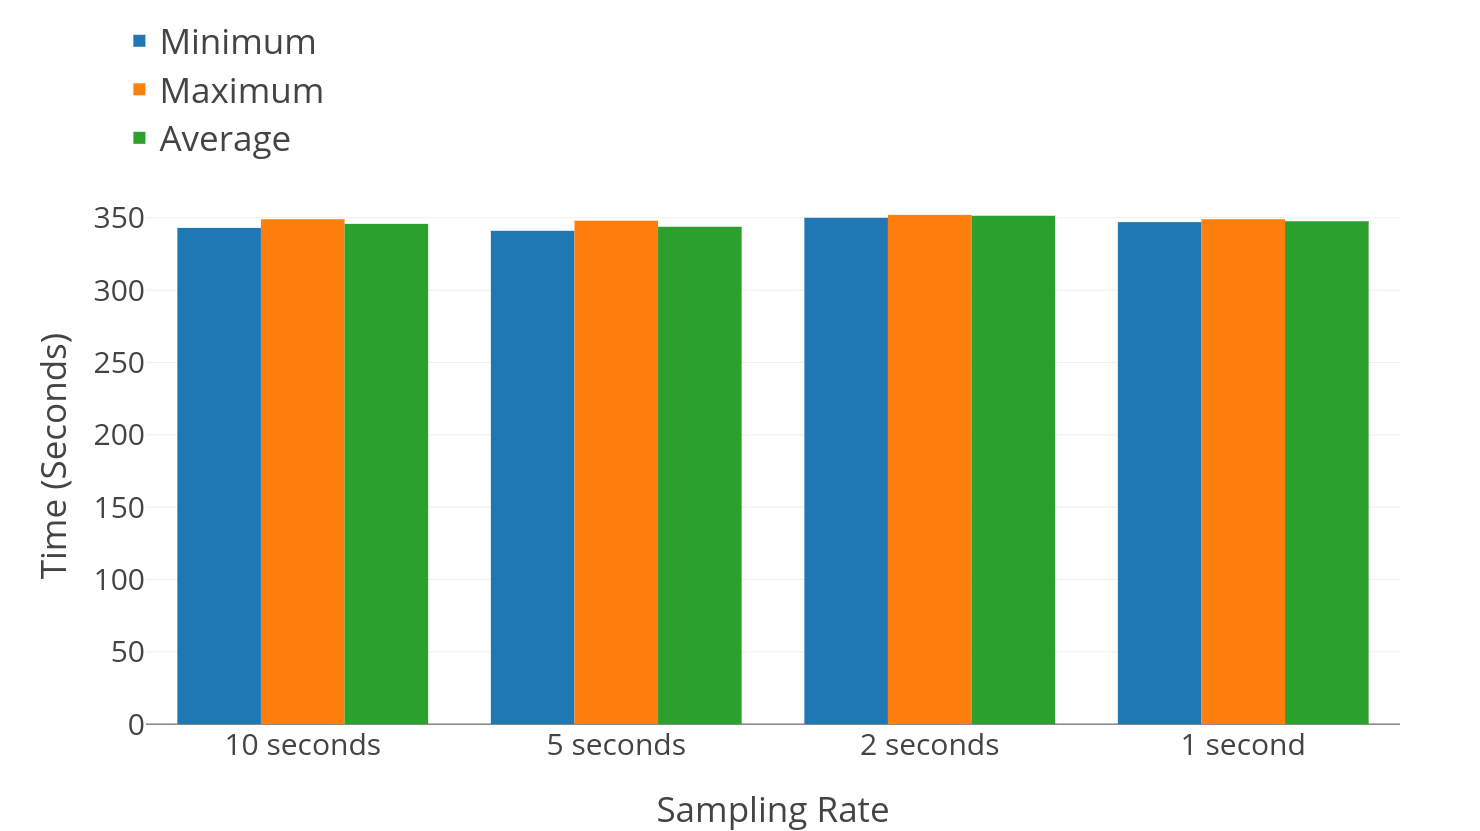
\includegraphics[width=\columnwidth,keepaspectratio,scale=1.0]{figures/MPI_T_Sampling_Frequently}
                \captionsetup{justification=centering}
                  \caption{Effect of MPI\_T sampling frequency on overhead for 3DStencil at 448 processes}
                   \label{fig:sampling_frequency}
        \end{figure*}
\end{center}
